\documentclass[tikz]{standalone}
\usepackage{tikz}
\usetikzlibrary{positioning, graphs}
\usetikzlibrary{graphs.standard}
\begin{document}
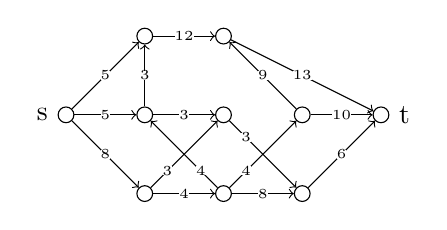
\begin{tikzpicture}
		[vertex/.style={draw,circle,inner sep = 0mm, minimum size = 2mm},
		 edgelabel/.style = {fill = white, inner sep = 0mm, font=\tiny}]
		\node[vertex, label = left : s] at (0,0) (s) {};
		\node[vertex] at (1,0) (b) {};
		\node[vertex] at (1,1) (c) {};
		\node[vertex] at (1,-1) (d) {};
		\node[vertex] at (2,0) (e) {};
		\node[vertex] at (2,-1) (f) {};
		\node[vertex] at (2,1) (g) {};
		\node[vertex] at (3,0) (h) {};
		\node[vertex] at (3,-1) (i) {};
		\node[vertex, label = right : t] at (4,0) (t) {};
		
		\draw[->] (s) to node[edgelabel] {$5$} (b);
		\draw[->] (s) to node[edgelabel] {$5$} (c);
		\draw[->] (s) to node[edgelabel] {$8$} (d);
		\draw[->] (b) to node[edgelabel] {$3$} (c);
		\draw[->] (b) to node[edgelabel] {$3$} (e);
		\draw[->] (c) to node[edgelabel] {$12$} (g);
		\draw[->] (d) to node[edgelabel, near start] {$3$} (e);
		\draw[->] (d) to node[edgelabel] {$4$} (f);
		\draw[->] (e) to node[edgelabel, near start] {$3$} (i);
		\draw[->] (f) to node[edgelabel, near start] {$4$} (b);
		\draw[->] (f) to node[edgelabel, near start] {$4$} (h);
		\draw[->] (f) to node[edgelabel] {$8$} (i);
		\draw[->] (g) to node[edgelabel] {$13$} (t);
		\draw[->] (h) to node[edgelabel] {$9$} (g);
		\draw[->] (h) to node[edgelabel] {$10$} (t);
		\draw[->] (i) to node[edgelabel] {$6$} (t);
		
\end{tikzpicture}
\end{document}